\documentclass{article}
\usepackage{tikz}
\usetikzlibrary{arrows.meta,positioning,calc,shapes.geometric}
\pagestyle{empty}
\begin{document}
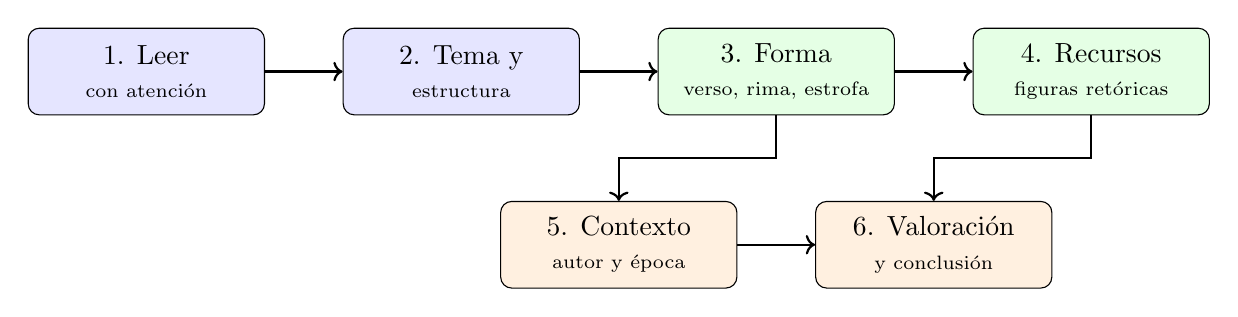
\begin{tikzpicture}
\tikzset{every node/.append style={align=center}}

\node[draw, rounded corners, fill=blue!10, minimum width=3.0cm, minimum height=1.1cm, align=center] (a) at (0,0) {1. Leer\\ \scriptsize con atención};
\node[draw, rounded corners, fill=blue!10, minimum width=3.0cm, minimum height=1.1cm, align=center] (b) at (4,0) {2. Tema y\\ \scriptsize estructura};
\node[draw, rounded corners, fill=green!10, minimum width=3.0cm, minimum height=1.1cm, align=center] (c) at (8,0) {3. Forma\\ \scriptsize verso, rima, estrofa};
\node[draw, rounded corners, fill=green!10, minimum width=3.0cm, minimum height=1.1cm, align=center] (d) at (12,0) {4. Recursos\\ \scriptsize figuras retóricas};
\node[draw, rounded corners, fill=orange!12, minimum width=3.0cm, minimum height=1.1cm, align=center] (e) at (6,-2.2) {5. Contexto\\ \scriptsize autor y época};
\node[draw, rounded corners, fill=orange!12, minimum width=3.0cm, minimum height=1.1cm, align=center] (f) at (10,-2.2) {6. Valoración\\ \scriptsize y conclusión};
\draw[->, thick] (a) -- (b); \draw[->, thick] (b) -- (c); \draw[->, thick] (c) -- (d);
\draw[->, thick] (d) -- ++(0,-1.1) -| (f);
\draw[->, thick] (e) -- (f);
\draw[->, thick] (c) -- ++(0,-1.1) -| (e);

\end{tikzpicture}
\end{document}
